\subsection[Ogólny mechanizm działania (Michał Krakowiak)]{Ogólny mechanizm działania}
Podłączenie urządzenia wykonującego do testowanego systemu powinno skutkować rozpoznaniem go jako tzw. Human Interface Device (dalej określanego jako HID). HID to klasa urządzeń korzystających z interfejsu USB do interakcji z człowiekiem (użytkownikiem komputera). Zazwyczaj wykorzystywane są do pobierania danych wejściowych oraz prezentacji danych wyjściowych \cite{oney}. Interfejs jest powszechnie stosowany przez producentów akcesoriów oraz dobrze udokumentowany w specyfikacji USB \cite{usbhid}.
Dzięki adopcji interfejsu popularne systemy takie jak Windows, Linux czy macOS są w stanie samodzielnie zidentyfikować nowe urządzenia i korzystać z nich bez potrzeby instalacji dedykowanych sterowników.
Ułatwia to pracę pentestera korzystającego z realizowanego systemu, ponieważ nie ma potrzeby tworzenia i dostarczenia własnych implementacji sterownika na każdy testowany system operacyjny (o ile nie ma w planach przygotowania niestandardowej funkcjonalności).
Urządzenia HID komunikują się z komputerem po przez blok danych nazywany raportem. Bity i bajty w nim sformatowane są w sposób określony w deskryptorze raportu.
\begin{lstlisting}[language={},caption={Przykładowy deskryptor odczytany z istniejącej klawiatury}]
Usage Page (Desktop),                   ; Generic desktop controls (01h)
Usage (Keyboard),                       ; Keyboard (06h, application collection)
Collection (Application),
    Usage Page (Keyboard),              ; Keyboard/keypad (07h)
    Usage Minimum (KB Leftcontrol),     ; Keyboard left control (E0h, dynamic value)
    Usage Maximum (KB Right GUI),       ; Keyboard right GUI (E7h, dynamic value)
    Logical Minimum (0),
    Logical Maximum (1),
    Report Size (1),
    Report Count (8),
    Input (Variable),
    Report Count (1),
    Report Size (8),
    Input (Constant),
    Report Count (3),
    Report Size (1),
    Usage Page (LED),                   ; LEDs (08h)
    Usage Minimum (01h),
    Usage Maximum (03h),
    Output (Variable),
    Report Count (5),
    Report Size (1),
    Output (Constant),
    Report Count (6),
    Report Size (8),
    Logical Minimum (0),
    Logical Maximum (255),
    Usage Page (Keyboard),              ; Keyboard/keypad (07h)
    Usage Minimum (None),               ; No event (00h, selector)
    Usage Maximum (FFh),
    Input,
End Collection
\end{lstlisting}
\textit{Można tu jeszcze opisać co znajduje się w podanym deskryptorze, co z tego wynika i dalej pisać o mechanizmie działania HID, a potem może trochę o plug and play, na ten moment nie starczyło czasu}
\begin{figure}[H]
    \centering
    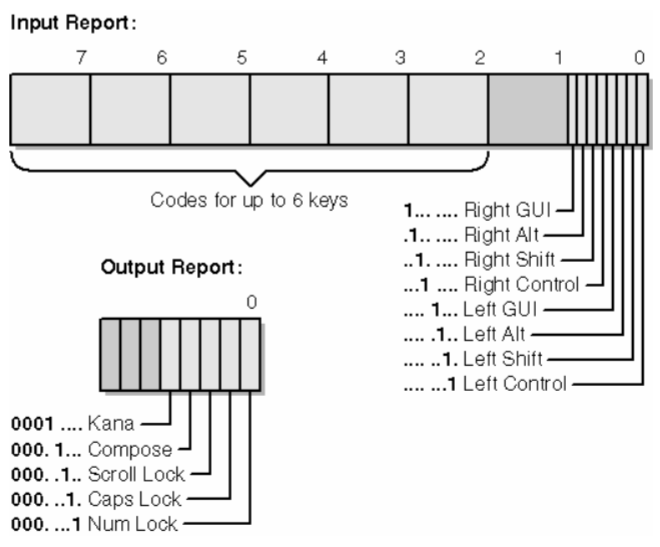
\includegraphics[width=\textwidth]{images/mk02.png}
    \caption{Struktura raportu \cite{oney}}
    \label{fig:report}
\end{figure}
